\documentclass[11pt]{article}

\usepackage[margin=1in]{geometry}
\usepackage{amsmath,amssymb}
\usepackage{graphicx}
\usepackage{booktabs}
\usepackage{caption}
\usepackage{microtype}
\usepackage[svgnames]{xcolor}
\usepackage[colorlinks=true,linkcolor=DarkBlue,urlcolor=DarkBlue,citecolor=DarkBlue]{hyperref}

\graphicspath{{figures/}}

\title{\textbf{Vector Compression for High-Dimensional Data}\\[0.4em]
\large A survey of linear-algebra compression methods with an honest retrieval evaluation}
\author{MATH 5110 --- Applied Linear Algebra\\
\href{https://github.com/claytomode/math5110-vector-compression}{\texttt{github.com/claytomode/math5110-vector-compression}}}
\date{}

\begin{document}
\maketitle

\begin{abstract}
\noindent
Modern AI systems store billions of high-dimensional vectors --- text embeddings, attention key/value caches, and retrieval indexes --- whose footprint scales as $n \cdot d \cdot (\text{bits per dimension})$. This paper surveys four classical linear-algebra tools for shrinking such vectors (Johnson--Lindenstrauss random projection, truncated SVD, 1-bit sign quantization, and uniform scalar quantization) and a recent two-stage method, TurboQuant, that combines scalar quantization with a quantized-JL residual correction. We implement pedagogical versions of each method in NumPy and evaluate them not only on geometric distortion but on a realistic retrieval task: a 1{,}380-chunk retrieval-augmented-generation (RAG) index built from a linear-algebra textbook, queried by 300 auto-generated questions and scored against full-precision ground truth. Our central finding is that \emph{distance preservation does not imply rank preservation}: Johnson--Lindenstrauss preserves pairwise geometry yet retains only 39\% of the true top-3 neighbors, while a two-line scalar quantizer at 4 bits retains 93\%. TurboQuant wins decisively at aggressive bit budgets (76\% vs 63\% top-3 overlap against scalar at matched stage-1 bits), but plain scalar quantization is the stronger choice once 4--8 bits per dimension are affordable. We argue that compression methods must be compared on \emph{measured} bits per dimension and on a \emph{retrieval} metric, not on nominal labels or distance error alone.
\end{abstract}

\section{Introduction}

A single OpenAI \texttt{text-embedding-3-small} vector at $d = 256$ dimensions costs $256 \times 32 = 8{,}192$ bits in \texttt{float32}. A modest corpus of one million chunks therefore costs roughly one gigabyte before any index structure is added, and production systems routinely store far more. The same arithmetic governs the attention key/value cache inside a running language model and the lookup table of token embeddings. In every case the cost is the product of three terms:
\begin{equation}
\text{storage} = n \cdot d \cdot (\text{bits per dimension}).
\end{equation}

Reducing any factor without destroying the geometry that downstream tasks depend on is the core problem of \textbf{vector compression}. The relevant geometry is almost always an inner product: retrieval ranks candidates by cosine similarity, and attention scores keys by dot product. When embeddings are L2-normalized, cosine similarity equals the dot product, so a compressor that approximately preserves inner products approximately preserves both ranking and attention.

This project has three parts, mirroring the course structure:
\begin{itemize}
  \item \textbf{Part 1 --- Survey.} The linear algebra of four compression families plus the TurboQuant pipeline.
  \item \textbf{Part 2 --- Computation.} NumPy implementations and two metric families: geometric distortion and retrieval overlap.
  \item \textbf{Part 3 --- Application.} A compressed textbook RAG index with a 300-query automatic evaluation and a live search UI.
\end{itemize}

\paragraph{Contributions.}
(1) A unified, from-scratch implementation of five compression methods sharing one embedding matrix and random seed. (2) An honest retrieval benchmark that uses full-precision top-$k$ as ground truth rather than synthetic labels. (3) A clear empirical separation between \emph{geometry-preserving} and \emph{rank-preserving} methods, with practical guidance on when each method wins.

\section{Background and theory}

Throughout, vectors live in $\mathbb{R}^d$. A query $q$ is scored against keys $k_1, \ldots, k_n$ by cosine similarity (equivalently, dot product after normalization). A compressor replaces each key with a cheaper representation whose scores $\hat{s}(q, k_i)$ approximate the true scores $s(q, k_i)$.

\subsection{Johnson--Lindenstrauss random projection}

The Johnson--Lindenstrauss (JL) lemma states that $n$ points in $\mathbb{R}^d$ can be linearly embedded into $\mathbb{R}^k$ with all pairwise distances preserved up to a factor of $(1 \pm \varepsilon)$, provided
\begin{equation}
k = O\!\left(\varepsilon^{-2} \log n\right).
\end{equation}
Critically, $k$ depends on the number of points and the tolerance, \emph{not} on the ambient dimension $d$. We use the standard Gaussian construction: a random matrix $R \in \mathbb{R}^{k \times d}$ with independent entries $R_{ij} \sim \mathcal{N}(0, 1/k)$, applied as a sketch
\begin{equation}
y = R x \in \mathbb{R}^k.
\end{equation}
The $1/\sqrt{k}$ scaling makes $R$ a near-isometry in expectation: $\mathbb{E}\,\|Rx\|^2 = \|x\|^2$. Because the map is linear and applied identically to keys and queries, inner products are preserved in expectation, and concentration of measure gives the $(1 \pm \varepsilon)$ guarantee with high probability.

\paragraph{How it works.} Each output coordinate $y_i = \sum_j R_{ij} x_j$ is a random weighted sum of all $d$ input coordinates. No single output depends on the data --- the matrix $R$ is drawn before seeing any vector --- yet averaging over $k$ independent random combinations makes the sketch length concentrate tightly around the true length, a law-of-large-numbers effect that sharpens as $k$ grows. This is why the required dimension depends only on the point count $n$ and the tolerance $\varepsilon$, never on the original dimension $d$: JL is a \emph{data-oblivious} compressor.

In our setting $d = 256$, $n = 1{,}380$, and a tolerance $\varepsilon = 0.3$ yields a target dimension of roughly $k \approx 128$, i.e. a nominal $2\times$ compression. The key conceptual point --- confirmed dramatically in our results --- is that \textbf{distance preservation is not rank preservation}. JL controls the magnitude of pairwise distances, but every sketch coordinate is a pure mixture, so the fine angular differences that separate near-duplicate neighbors are buried under projection noise. The lemma promises the \emph{size} of distances, not the \emph{order} of the nearest neighbors, and top-$k$ retrieval needs the order.

\subsection{Truncated (rank-\texorpdfstring{$k$}{k}) SVD}

The singular value decomposition factors the stacked embedding matrix $A \in \mathbb{R}^{n \times d}$ as $A = U \Sigma V^\top$ and truncates to the top $k$ singular directions:
\begin{equation}
A_k = U_k \Sigma_k V_k^\top.
\end{equation}
The right singular vectors $V_k \in \mathbb{R}^{d \times k}$ span the $k$-dimensional subspace of maximum variance across the corpus. Each vector is compressed by projection into that subspace and reconstructed back into $\mathbb{R}^d$:
\begin{equation}
z = V_k^\top x \in \mathbb{R}^k, \qquad \hat{x} = V_k V_k^\top x.
\end{equation}
\paragraph{How it works.} Where JL is data-oblivious, SVD is data-optimal: it spends its $k$ dimensions on exactly the directions in which the corpus actually varies. The top singular vectors are the principal axes of the cloud of embeddings, and projecting onto them keeps the most ``energy'' (variance) recoverable from $k$ numbers. By the Eckart--Young theorem, $A_k$ is the optimal rank-$k$ approximation of $A$ in both the Frobenius and spectral norms --- no other linear rank-$k$ compressor achieves smaller reconstruction error.

Two caveats temper this optimality in practice. First, the basis $V_k$ must be fit on the full corpus in advance, so out-of-distribution vectors lose alignment, and a query's relevant signal may live partly in the discarded tail --- which is why aggressive truncation (rank-8, rank-16) shows the largest distance error in our results. Second, storage is not simply $k$ floats per vector: the shared basis $V_k$ and the per-vector coefficients both count, so the \emph{measured} compression ratio is lower than the nominal $d/k$. For $k = 64$ the nominal ratio is $4\times$, but amortized storage yields about $3.4\times$.

\subsection{Sign (1-bit) quantization and QJL scoring}

The most aggressive linear compressor keeps only the sign of each coordinate:
\begin{equation}
\hat{x} = \operatorname{sign}(x) \in \{-1, +1\}^d,
\end{equation}
collapsing 32 bits per coordinate to 1, a nominal $32\times$ reduction. Scoring against a full-precision query recovers an estimate of the inner product. The quantized-JL (QJL) refinement first applies a random rotation $R$, then quantizes; the angle between rotated sign vectors encodes the original cosine similarity:
\begin{equation}
\operatorname{score}(q, \hat{x}) = \frac{\operatorname{sign}(Rx)^\top (Rq)}{\sqrt{d}} \approx \cos(x, q).
\end{equation}
\paragraph{How it works.} Recording $\operatorname{sign}(x)$ stores which side of each coordinate axis --- or, after a random rotation, each random hyperplane --- the vector falls on. Two vectors pointing in similar directions agree on most of these signs, so the number of \emph{agreeing bits} (a Hamming distance) is a cheap estimator of the angle between them; this is the same idea as sign-random-projection locality-sensitive hashing. One bit per coordinate localizes direction coarsely and cheaply, but it cannot distinguish vectors that already sit close together on the sphere: sign quantization works well when relevant vectors are well separated, and it fails when the true top-$k$ items cluster tightly --- exactly the regime where retrieval needs the most angular precision.

\subsection{Uniform scalar quantization}

Scalar quantization divides each coordinate's range into $2^b$ equal buckets and rounds to the nearest bucket center. With per-coordinate range $[x_{\min}, x_{\max}]$ the step size is
\begin{equation}
\Delta = \frac{x_{\max} - x_{\min}}{2^b - 1},
\end{equation}
and the worst-case rounding error per coordinate is $\Delta/2$, giving the reconstruction bound
\begin{equation}
\|x - \hat{x}\|^2 \le d \cdot \left(\frac{\Delta}{2}\right)^2.
\end{equation}
Each additional bit halves $\Delta$ and therefore halves the per-coordinate error, producing a clean and predictable quality-versus-bits tradeoff. The compression ratios are exact: $b = 8$ gives $4\times$, $b = 4$ gives $8\times$, and $b = 2$ gives $16\times$.

\paragraph{How it works.} Scalar quantization is the most direct method: keep every coordinate, just store it coarsely on a per-dimension grid. Because it never mixes coordinates, it adds no projection noise of the kind JL suffers --- only independent rounding error that shrinks geometrically with the bit budget. That is why it is such a strong baseline: by 4 bits the grid is already fine enough that the cosine ranking of neighbors is barely perturbed, and at 8 bits it is effectively lossless. Its weakness shows only at 2 bits, where the grid is coarse and the rounding error is \emph{correlated} across a vector's coordinates, systematically nudging its direction --- precisely the bias that TurboQuant's residual stage is designed to remove. As our results show, scalar quantization at 4--8 bits matches or beats far more elaborate methods.

\subsection{TurboQuant: a two-stage pipeline}

TurboQuant (Google Research, ICLR 2026) combines scalar quantization with a JL-style residual correction. We implement a pedagogical version on course embeddings. The pipeline has three steps:
\begin{itemize}
  \item \textbf{Stage 0 --- Rotate.} A cheap random rotation (coordinate permutation plus Rademacher signs) flattens the geometry so that no axis carries disproportionate energy before quantization. The rotation metadata is $O(d)$, not $O(d^2)$.
  \item \textbf{Stage 1 --- Quantize.} Uniform scalar quantization with $b$ bits per coordinate in the rotated space produces a coarse reconstruction $\hat{x}_1$.
  \item \textbf{Stage 2 --- 1-bit residual.} The residual $r = x - \hat{x}_1$ is captured with a single sign bit per coordinate under a QJL transform.
\end{itemize}
Scoring uses the full-precision query on both stages, so the residual term corrects the stage-1 bias at essentially zero additional storage:
\begin{equation}
\operatorname{score}(q, x) \approx q^\top \hat{x}_1 + \frac{\|r\| \cdot \operatorname{sign}(Rr)^\top (Rq)}{\sqrt{d}}.
\end{equation}
The residual $r$ is small in norm, so a coarse 1-bit JL sketch of it is enough to remove most of the quantization bias.

\paragraph{How it works.} TurboQuant is best read as a correction layer bolted onto scalar quantization. The rotation (Stage 0) destroys any coordinate system in which energy is concentrated on a few axes, so the uniform grid of Stage 1 wastes no resolution; this is what lets the stage-1 quantizer run at an aggressive 2--3 bits. Stage 1 then leaves behind a structured error --- the same correlated, direction-biasing residual that hurts plain scalar quantization at low bit budgets. The insight is that this residual, while not negligible, is \emph{small in norm and roughly isotropic} after rotation, so it is exactly the kind of vector a cheap 1-bit JL sketch estimates well. Spending one extra bit per coordinate to recover the residual's contribution to the inner product removes most of the stage-1 bias without storing the residual itself. The payoff is largest precisely where scalar quantization is weakest (2--3 bits) and vanishes once the stage-1 grid is already fine (4+ bits), where the rotation and residual become pure overhead.

The cost is honesty about bits: a method labeled ``TQ-2'' actually consumes about $3.2$ bits per dimension (two stage-1 bits, one residual bit, plus amortized rotation and norm metadata), not the nominal $2.0$. This distinction is essential when comparing methods.

\section{Methods and experimental setup}

\subsection{Corpus and embeddings}

The retrieval corpus is the source text of Professor He Wang's MATH 5110 textbook, \emph{Advanced Linear Algebra for AI}, pulled directly from its public Quarto (\texttt{.qmd}) repository. Chapters are split on section boundaries and then into overlapping character windows (900 characters per chunk, 120-character overlap), yielding \textbf{1{,}380 chunks}. Each chunk is embedded with \texttt{text-embedding-3-small} at $d = 256$. Retrieval is ranked by \textbf{cosine similarity} throughout --- the scoring functions normalize vectors at comparison time --- so ranking depends on direction, not magnitude.

\subsection{Evaluation queries and metric}

We auto-generate \textbf{300 stratified queries} by sampling across chunks (using section titles and leading sentences) so that every part of the book is represented, with a fixed seed for reproducibility. For each query, the \textbf{full-precision top-$k$ set is the ground truth} (100\% by definition). A compressed index is scored by
\begin{equation}
\text{overlap@}k = \frac{\bigl|\,\mathrm{TopK}_{\text{full}} \cap \mathrm{TopK}_{\text{comp}}\,\bigr|}{k}.
\end{equation}
This is recall of the true neighbors, and because it is a set intersection it is rank-blind within the top-$k$ window --- appropriate when a language model consumes any of the retrieved passages, not only the first. We report $k = 3$ for RAG and $k = 10$ for the token study. We also report \textbf{mean relative pairwise distance error} to measure geometry directly, and a \textbf{drift breakdown} classifying each query as a perfect match, partial drift, or zero overlap.

\paragraph{Two different geometries.} It is worth being explicit that our two quality measures use \emph{different} notions of closeness, and they are not interchangeable. The geometric-distortion metric is built on \textbf{Euclidean ($L_2$) distance}: for each method we compute mean relative pairwise distance error, $\bigl|\,\|x_i - x_j\| - \|c(x_i) - c(x_j)\|\,\bigr| / \|x_i - x_j\|$ averaged over pairs, which is exactly the quantity the Johnson--Lindenstrauss lemma bounds. Retrieval, by contrast, ranks neighbors by \textbf{cosine similarity}, which depends only on the \emph{angle} between vectors. Because our embeddings are not unit-normalized before compression, these two views do not coincide: $L_2$ distance mixes angle and magnitude, while cosine discards magnitude entirely. A compressor can therefore shrink Euclidean distance error while still scrambling the angular order that retrieval depends on --- which is precisely the JL story below. We deliberately report both so the gap between ``preserving geometry'' and ``preserving rankings'' is visible rather than assumed away.

\subsection{Implementation}

All methods are implemented from scratch in NumPy, sharing one embedding matrix and one random seed. The compression families and the bit/dimension ladders evaluated are: \texttt{full\_precision}; \texttt{jl\_\{16,32,64,128\}}; \texttt{rank\_\{8,16,32,64\}}; \texttt{sign\_1bit}; \texttt{scalar\_\{2,3,4,8\}bit}; and \texttt{turboquant\_\{2,3,4,8\}bit}. The same scoring functions back a FastAPI + SvelteKit web application that lets a user search the book and compare indexes side by side.

\section{Results}

\subsection{Geometric distortion}

Figure~\ref{fig:distance} reports mean relative pairwise \emph{Euclidean} distance error (lower is better). The 8-bit methods are effectively lossless --- \texttt{turboquant\_8bit} at $0.0002$ and \texttt{scalar\_8bit} at $0.0003$ are indistinguishable from full precision at $0.0000$. The largest distortions come from aggressive rank truncation: \texttt{rank\_16} and \texttt{rank\_8} sit at the high end because discarding singular directions removes real signal that the inner product depends on. This figure measures geometry only; the next two figures show that good geometry does not guarantee good retrieval.

\begin{figure}[htbp]
  \centering
  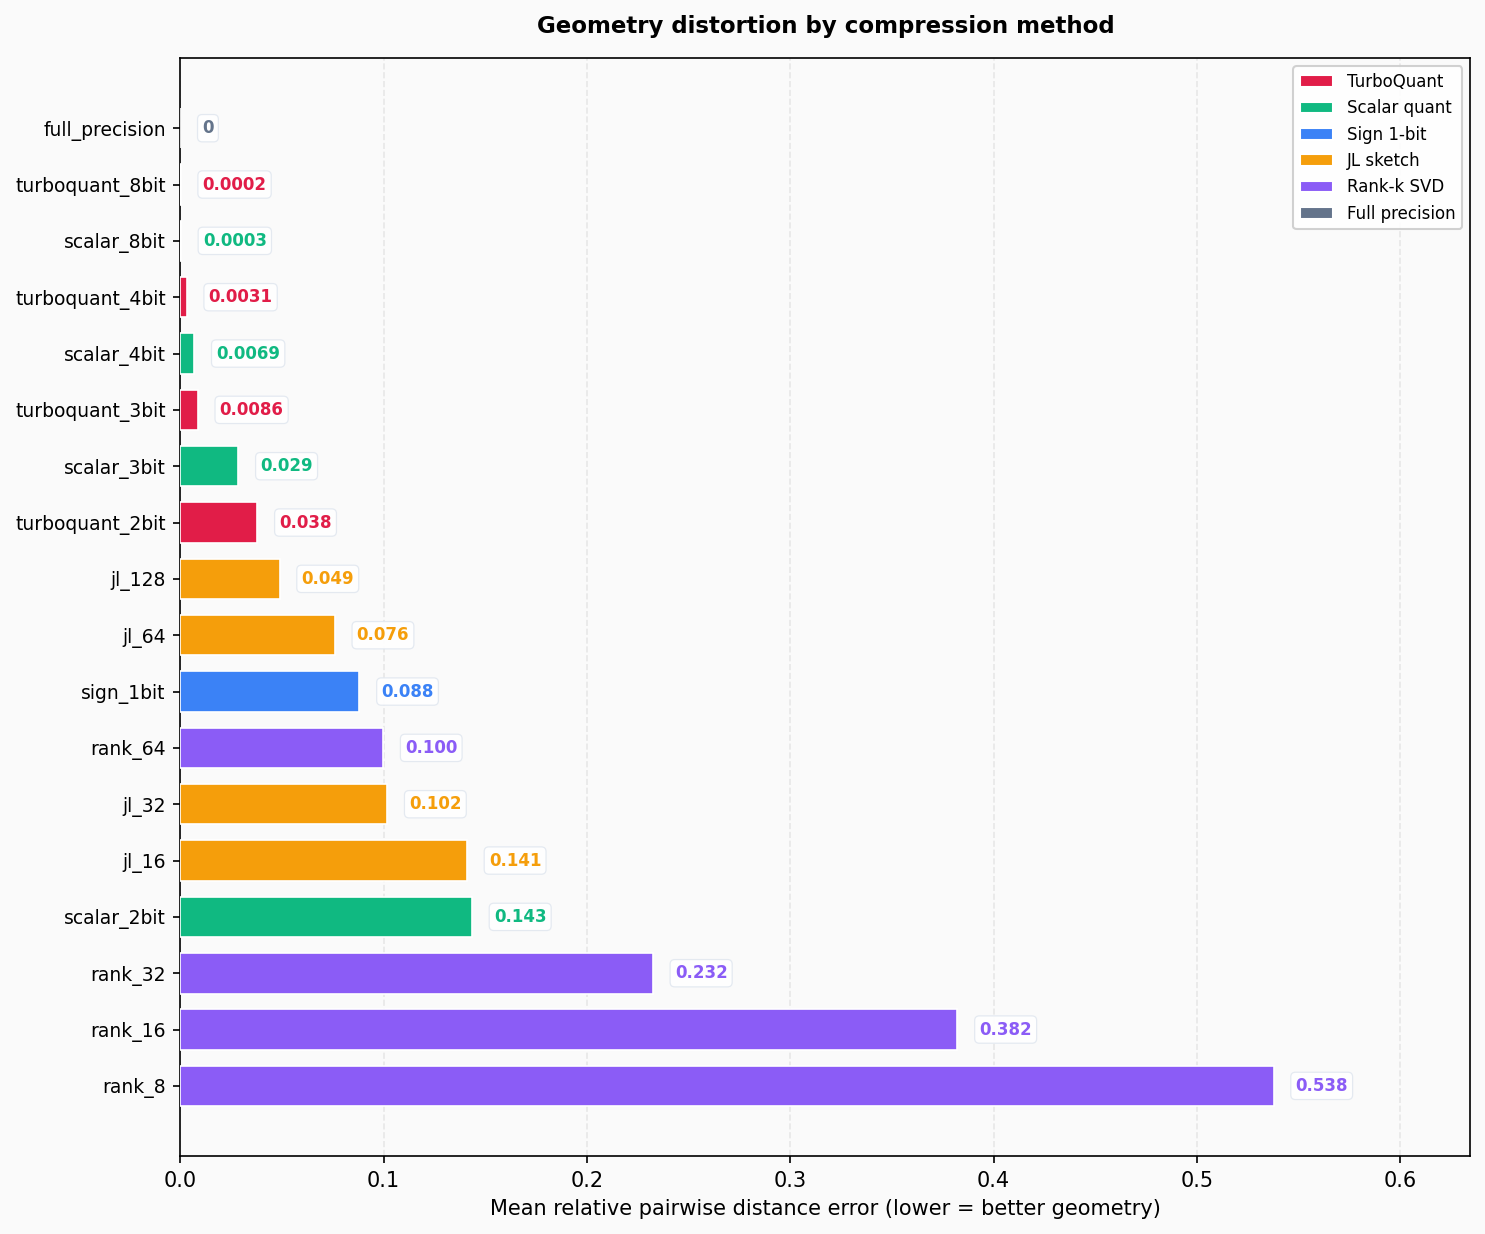
\includegraphics[width=0.9\textwidth]{distance_error.png}
  \caption{Mean relative pairwise distance error by method (lower is better).}
  \label{fig:distance}
\end{figure}

\subsection{RAG compression frontier}

Figure~\ref{fig:frontier} plots top-3 overlap (accuracy) against compression ratio, with the Pareto frontier traced in red. The headline numbers, taken from \texttt{python/data/presentation\_results.json}, are given in Table~\ref{tab:rag}.

\begin{table}[htbp]
  \centering
  \caption{RAG retrieval results (300 queries, $k = 3$, 1{,}380 chunks).}
  \label{tab:rag}
  \begin{tabular}{lrrr}
    \toprule
    Method & Top-3 overlap & Bits/dim (measured) & Compression \\
    \midrule
    Full precision    & 100.0\% & 32.0 & $1.0\times$ \\
    JL-128            & 39.2\%  & 16.0 & $2.0\times$ \\
    Rank-64           & 64.8\%  & 9.5  & $3.4\times$ \\
    Sign 1-bit        & 47.9\%  & 1.1  & $28.4\times$ \\
    Scalar 2-bit      & 62.8\%  & 2.0  & $16.0\times$ \\
    TurboQuant 2-bit  & 76.1\%  & 3.2  & $10.1\times$ \\
    Scalar 3-bit      & 82.4\%  & 3.0  & $10.7\times$ \\
    TurboQuant 3-bit  & 87.0\%  & 4.2  & $7.7\times$ \\
    Scalar 4-bit      & 93.2\%  & 4.0  & $8.0\times$ \\
    TurboQuant 4-bit  & 93.3\%  & 5.2  & $6.2\times$ \\
    Scalar 8-bit      & 99.7\%  & 8.0  & $4.0\times$ \\
    TurboQuant 8-bit  & 99.8\%  & 9.2  & $3.5\times$ \\
    \bottomrule
  \end{tabular}
\end{table}

Two facts dominate the frontier. First, the JL points (\texttt{jl\_128}, \texttt{jl\_64}) fall far below it: despite strong distance guarantees, they are the worst retrievers per bit. Second, the choice between TurboQuant and scalar depends on the budget. At aggressive stage-1 bits the residual correction is decisive --- TurboQuant 2-bit reaches 76.1\% versus scalar 2-bit at 62.8\%, a 13-point gain. Once 4 bits are affordable the methods tie on accuracy (93.3\% vs 93.2\%), and scalar wins on the frontier because it avoids TurboQuant's rotation and residual overhead.

\begin{figure}[htbp]
  \centering
  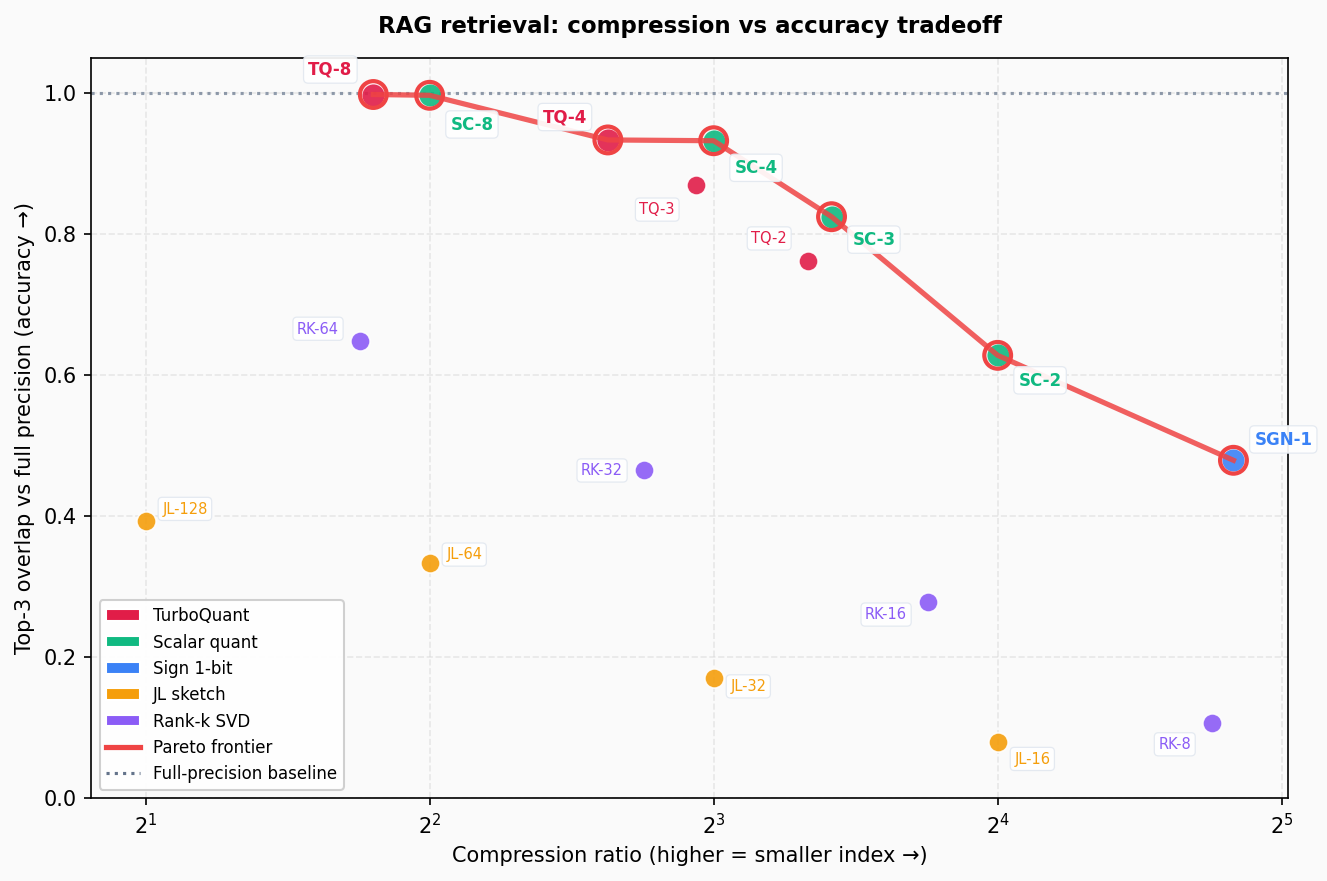
\includegraphics[width=0.9\textwidth]{rag_compression_frontier.png}
  \caption{RAG compression frontier: top-3 overlap vs compression ratio (upper-right is better).}
  \label{fig:frontier}
\end{figure}

\subsection{Retrieval drift}

Figure~\ref{fig:drift} decomposes the 300 queries into perfect top-$k$ matches, partial drift, and zero-overlap failures. High-bit scalar and TurboQuant configurations keep nearly all queries in the perfect-match band, whereas \texttt{rank\_8} and \texttt{jl\_16} are dominated by partial drift and outright failures. Drift concentrates on queries where several chunks have nearly equal scores: small quantization noise reorders a close top-3, which is precisely the failure mode that the QJL residual mitigates at low bit budgets.

\begin{figure}[htbp]
  \centering
  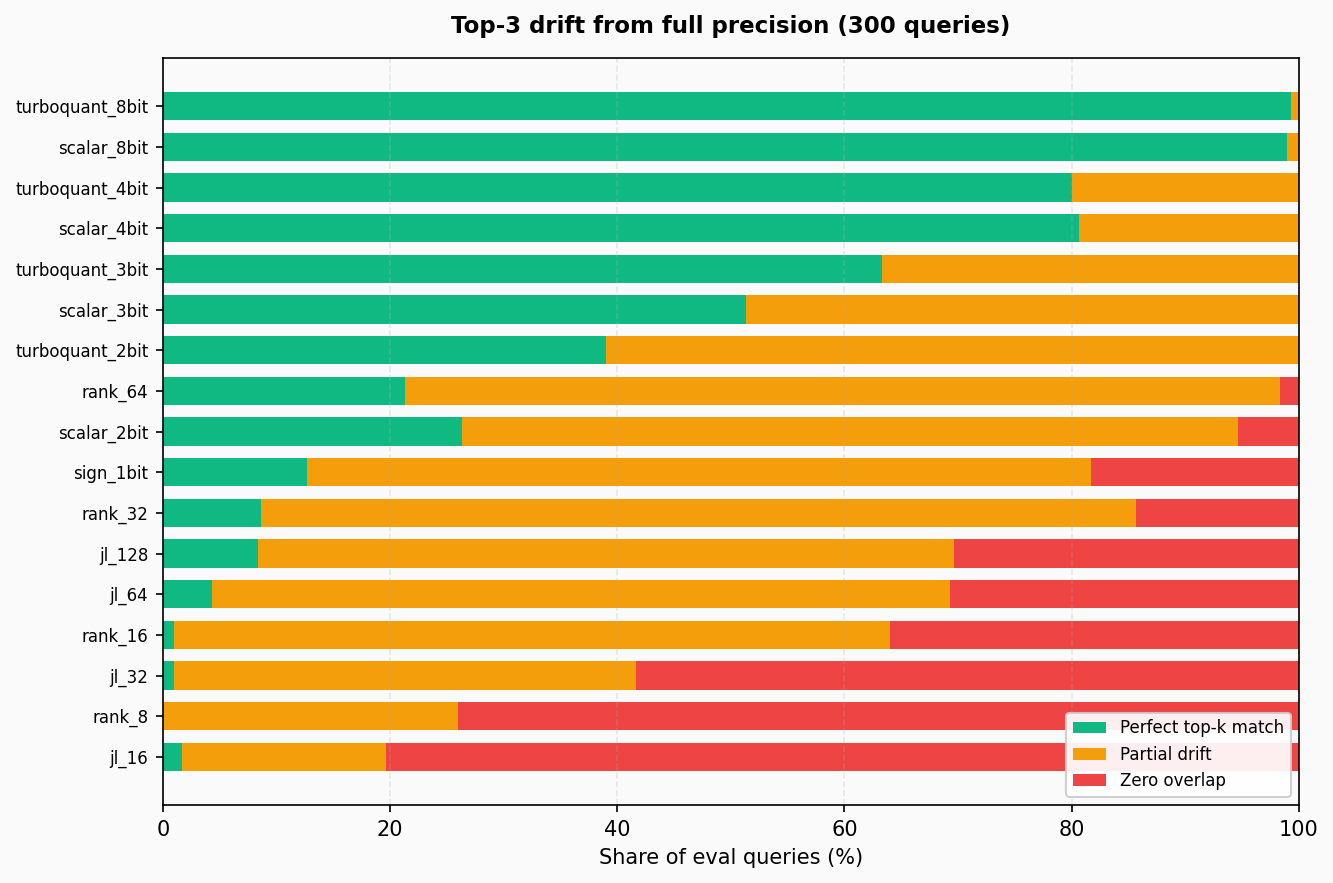
\includegraphics[width=0.9\textwidth]{rag_drift_summary.png}
  \caption{RAG top-$k$ drift from full precision across the 300 evaluation queries.}
  \label{fig:drift}
\end{figure}

\subsection{Token study (cross-check)}

On a smaller, easier token-embedding task (recall@10), the ordering is the same: TurboQuant leads scalar at matched stage-1 bits (87.0\% vs 82.5\% at 2 bits; 94.8\% vs 90.7\% at 3 bits) and the gap closes by 4 bits (97.2\% vs 95.8\%). This consistency across two corpora supports the conclusions below rather than attributing them to one dataset.

\section{Discussion}

\paragraph{TurboQuant wins when bits are scarce.} When the stage-1 budget is 2--3 bits, scalar quantization is badly biased and the JL residual correction is worth its overhead. TurboQuant 2-bit beats scalar 2-bit by 13 points of top-3 overlap, turning a 1-bit-class method (\texttt{sign\_1bit} at 47.9\%) into a usable retriever (76.1\%).

\paragraph{Scalar wins when bits are plentiful.} At 4--8 bits the stage-1 quantizer is already accurate, the residual contributes little, and the rotation plus residual metadata are pure overhead. Scalar 4-bit matches TurboQuant 4-bit on accuracy while using fewer total bits, making it the better engineering choice when storage allows.

\paragraph{Distance theory is not retrieval theory.} This is the project's sharpest lesson. JL has the strongest theoretical guarantee of any method here, yet \texttt{jl\_128} retrieves only 39\% of the true top-3. The lemma preserves the \emph{magnitude} of pairwise distances, but top-$k$ retrieval depends on their \emph{order}, and a near-isometry can still permute close neighbors. Geometry preservation is necessary but not sufficient for ranking.

\paragraph{Labels are not bit budgets.} A method's name encodes a design parameter, not its true cost. TurboQuant 2-bit consumes about 3.2 bits per dimension once residual and metadata are counted, and rank-$k$ stores a shared basis on top of per-vector coefficients. Fair comparison requires plotting against \emph{measured} bits per dimension, which is why every table here reports it.

\section{Limitations}

This study uses one corpus, one embedding model, and one automatically generated query set; absolute numbers will shift with domain, dimension, and query distribution. The TurboQuant implementation is pedagogical: it uses a lightweight permutation-and-sign rotation rather than a full structured transform, and omits learned codebooks and the polar-coordinate machinery of the full method. We evaluate retrieval overlap, not end-to-end generation quality, and we do not reproduce language-model KV-cache inference --- the shared object of study is the linear algebra of compressed inner-product search, not the inference stack.

\section{Conclusion}

Vector compression is governed by a single product, $n \cdot d \cdot (\text{bits per dimension})$, and by a single geometric requirement, approximate preservation of inner products. We surveyed four classical methods and one modern two-stage pipeline, implemented them from scratch, and evaluated them on a realistic textbook RAG task with full-precision ground truth. The results draw a clean line between geometry and ranking: Johnson--Lindenstrauss preserves distances but not retrieval order, sign quantization is extreme but brittle, truncated SVD is optimal in reconstruction yet costly to store, and scalar quantization is a deceptively strong baseline. TurboQuant's quantized-JL residual earns its overhead only at aggressive bit budgets, where it converts a 1-bit-class compressor into a competitive retriever. The practical recommendation is concise: choose TurboQuant when you must compress below 4 bits per dimension, choose scalar quantization otherwise, and always compare methods on measured bits per dimension against a retrieval metric --- never on nominal labels or distance error alone.

\begin{thebibliography}{9}

\bibitem{jl1984} Johnson, W. B., \& Lindenstrauss, J. (1984). Extensions of Lipschitz maps into a Hilbert space. \emph{Contemporary Mathematics}, 26, 189--206.
\bibitem{dasgupta2003} Dasgupta, S., \& Gupta, A. (2003). An elementary proof of a theorem of Johnson and Lindenstrauss. \emph{Random Structures \& Algorithms}, 22(1), 60--65.
\bibitem{eckart1936} Eckart, C., \& Young, G. (1936). The approximation of one matrix by another of lower rank. \emph{Psychometrika}, 1(3), 211--218.
\bibitem{rag2020} Lewis, P., et al. (2020). Retrieval-augmented generation for knowledge-intensive NLP tasks. \emph{NeurIPS}.
\bibitem{qjl2025} Zandieh, A., et al. (2025). Quantized Johnson--Lindenstrauss transforms (QJL). \emph{AAAI}. \href{https://arxiv.org/abs/2406.03482}{arXiv:2406.03482}.
\bibitem{polarquant2026} Zandieh, A., et al. (2026). PolarQuant: Quantizing the KV cache with polar coordinates. \emph{AISTATS}. \href{https://arxiv.org/abs/2502.02617}{arXiv:2502.02617}.
\bibitem{turboquant2026} Zandieh, A., Mirrokni, V., et al. (2026). TurboQuant: KV cache compression with polar and quantized Johnson--Lindenstrauss transforms. \emph{ICLR}. \href{https://arxiv.org/abs/2504.19874}{arXiv:2504.19874}.
\bibitem{turboquantblog} Google Research (2026). \href{https://research.google/blog/turboquant-redefining-ai-efficiency-with-extreme-compression/}{TurboQuant: Redefining AI efficiency with extreme compression}.
\bibitem{openai} OpenAI. \href{https://platform.openai.com/docs/guides/embeddings}{Embeddings guide} --- \texttt{text-embedding-3-small}, $d = 256$.

\end{thebibliography}

\end{document}
